\documentclass[12]{article}
\usepackage[margin=1.0in]{geometry}
\usepackage[utf8]{inputenc}
\usepackage{titlesec}
\usepackage{physics}
\usepackage{graphicx}
\usepackage{siunitx}
\usepackage{cancel}
\usepackage{amsmath}
\usepackage{textcomp}
\usepackage{gensymb}
\usepackage{natbib}
\usepackage{bm}
\usepackage{setspace}
\usepackage[version=4]{mhchem}

\titleformat*{\subsection}{\normalfont\fontfamily{phv}}
%\titleformat*{\subsection}[runin]{}{}{}{}[]
  \titleformat{\subsection}[runin]{\normalfont\bfseries}{\thesubsection.}{3pt}{}
  \titleformat{\subsubsection}[runin]{\normalfont\bfseries}{\thesubsubsection.}{3pt}{}

\title{{\textsc{\Large Antarctic Radiation}}}
\author{\textsc{Lyssa Freese}
\\\\
Advised by Prof. Tim Cronin}
\doublespacing
\begin{document}
\maketitle
\thispagestyle{empty}

\setlength{\leftskip}{1.1cm}
\setlength{\rightskip}{1.1cm}


\bigskip
\bigskip

{\textsc{Abstract.} }
Greenhouse gases (GHG), such as \ce{CO2}, impact global and local outgoing longwave radiation (OLR). The Antarctic is known for its a strong temperature inversion, where the addition of GHG can lead to increased OLR due to higher radiating temperatures higher in the atmosphere. Here we develop a radiative-advective-turbulence single-column model based on observed temperatures at the South Pole and timestep it forward under different \ce{CO2} concentrations. We discuss 1. initial conditions under varying \ce{CO_2} concentrations and 2. variation of temperature and radiative fluxes as we timestep the model forward under a normal and doubled \ce{CO_2} scenario. We confirm that there is negative TOA forcing with increased \ce{CO_2} during all seasons but austral winter. Despite this negative forcing, we also find increased temperatures at the surface across all seasons, and cooling in the stratosphere with a doubling of \ce{CO_2}.
\bigskip
\bigskip 
\clearpage
\setcounter{page}{1}

\setlength{\leftskip}{0cm}
\setlength{\rightskip}{0cm}

\section{Introduction}
The Antarctic is characterized by a strong, year-round temperature inversion in the bottom 1 kilometer of the atmosphere. This is in contrast to the rest of the planet, such that surface temperatures, particularly in the central part of the continent, are colder than atmospheric temperatures just above them\citep{hudson_look_2005}. As emissions of \ce{CO_2} continue to rise due anthropogenic sources, the role that greenhouse gases (GHG) play in local Antarctic radiative balance, where such a temperature inversion is present, are important to consider.

Previous work has found that GHG emissions under a temperature inversion cause atmospheric longwave radiation to be less than the surface longwave emissions. This in turn leads to an increase in outgoing longwave radiation (OLR), and a cooling of the Antarctic atmosphere, due to radiative effects alone\citep{schmithusen_how_2015}. This was seen in a two-box model, line-by-line radiative transfer calculations, and experiments with the European Centre for Medium-Range Weather Forecast (ECMWF) atmospheric model. These conclusions; however, do not describe the impact that GHG have on surface temperature or the structure of the atmospheric column temperature. In order to investigate the implications that chlorofluorocarbons (CFCs) would have in the Antarctic, \cite{flanner_climate_2018} utilize Community Earth System Model (CESM), a fully coupled atmosphere, ocean, and land model, to model the surface and atmospheric temperature response. This work finds warming surface temperatures, and cooling in the layer in which CFCs were emitted. Theoretical work utilizing a grey gas model similarly found increasing surface temperatures in response to increased optical depth in a high latitude scenario \citep{payne_conceptual_2015}.

We aim to bring together much of this work by developing a single-column radiative-advective model rooted in observations, in order to build upon the theoretical findings in high latitude scenarios, and to investigate surface, column and top of atmosphere (TOA) response to increased levels of \ce{CO_2} both initially, and over time. We analyze 1) the surface, column, and top of atmosphere (TOA) radiative and temperature responses to different \ce{CO_2} levels at an initial time and 2) the changes in these responses over the span of three months. We find that OLR responses are dependent upon season, surface net longwave fluxes decrease with increasing GHG concentration, and that surface temperature and OLR under higher GHG concentrations are larger after 3 months.


\section{Methods}
\subsection{Temperature and gas data}
 To create monthly column gas and temperature profiles (\ref{fig:temperature_profiles}), we utilize monthly average temperature profiles from the South Pole station, modified according to Schmithüsen et al., as well as yearly average ozone volumetric mixing ratio (vmr), and water vapor vmr (w) from their work \citep{schmithusen_how_2015}. The column specific humidity is calculated at every level using
\begin{equation}
    q = w/1+w
\end{equation}

 We adjust the lowest levels of the temperature, ozone, and specific humidity profile to measure one reading every 100m in order to satisfy the CFL condition of $\frac{\kappa_0*timestep}{dz^2_{surf}}$, where our timestep is one hour. Six column CO2 profiles are created, at 0, 100, 200, 380, 760, 1000, and 1500 ppm, in order to give a full range of responses to different values. 

\begin{figure}[htb!]
\noindent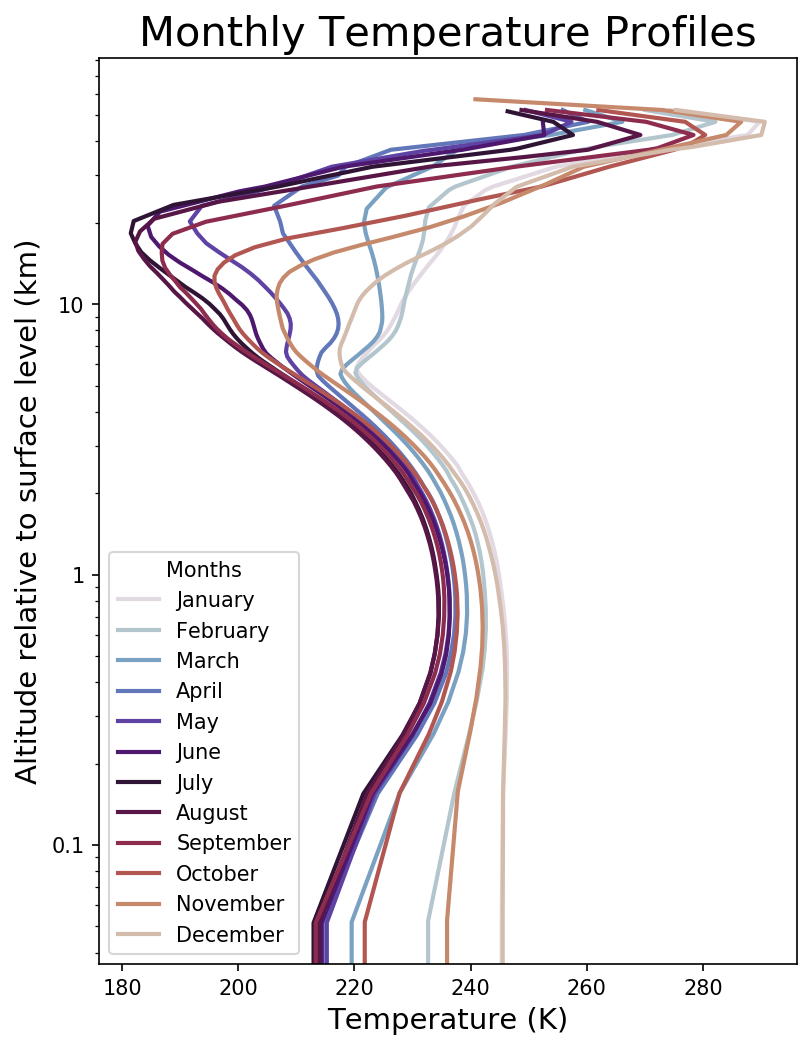
\includegraphics[width=.5\textwidth]{figures/initial_temperature_profiles.png}
\centering
\caption{Initial monthly temperature profiles as created by Schmithüsen et al.}
\label{fig:temperature_profiles}
\end{figure}

\subsection{Model Setup}
We utilize these monthly temperature profiles in a single column model in CLIMLAB \citep{rose_climlab_2018}, an open source python climate model. We adjust the solar insolation to a monthly mean insolation, to capture the variability in shortwave radiation in summer and winter seasons in the Antarctic. 

Our single-column model is comprised of three parts: a radiative, an advective, and a turbulent component. The radiation is calculated utilizing an RRTMG radiation scheme (\linkhttp{http://rtweb.aer.com/rrtm\_frame.html}). 

We construct an exponentially decaying turbulent component according to
\begin{equation}
    F_{turb} = -\kappa_0*exp(-\frac{z}{d})*\frac{d\theta}{dz}
\end{equation}
Where $\kappa_0$ is a surface turbulent diffusivity, scaled exponentially over the height of the column, and $d$ is a scale factor of 100 meters. We calculate an initial monthly $\kappa_0$ as
\begin{equation}
    \kappa_0 = \frac{F_{sfc, rad}}{\frac{d\theta}{dz}_{sfc}}
\end{equation}
Where $F_{sfc, rad}$ is the surface shortwave flux minus the surface longwave flux, as we assume the total flux at the surface boundary is equal to zero. From this, we average the (nine) positive $\kappa_0$ values, and use this as our final $\kappa_0$ throughout the experiments.

The turbulent heating rate is thus the flux divergence times the specific heat and density of air and ice, for the atmosphere and surface, respectively.

\begin{equation}
    HR_{turb} = \frac{dF_{turb}}{dz} * c_p * \rho
\end{equation}

We calculate our advective heating rate based on the initial state for each month at \ce{CO_2} = 380ppm, where it is set to equilibrate the sum of the radiative and turbulent heating rates.

\begin{equation}
    \frac{dF_{adv}}{dy} = -(\frac{dF_{rad}}{dz} + \frac{dF_{turb}}{dz})
\end{equation}

This is held constant throughout time, in order to allow us to look at the adjustments of the radiative and turbulent components in time, based on an initial state. 

We run the model forward for 3 months to assess the change over time in different \ce{CO_2} scenarios, in which we look at 380ppm as a base case, and 760ppm as our doubled \ce{CO_2} scenario. We look at the December and June scenarios to represent the austral summer and winter, respectively.

\section{Results}
\subsection{Initial State}
In our initial state, we see a clear temperature inversion as in \ref{fig:temperature_profiles}, as expected, across all months !!!***\cite[{}. This inversion is stronger during the austral winter when surface warming from shortwave radiation is at a low. 

The initial conditions under each of our column \ce{CO_2} concentrations show variations in OLR, surface net longwave flux, and surface net shortwave flux. OLR (\ref{fig:init_OLR}) increases with atmospheric \ce{CO_2} concentration in December, but decreases with \ce{CO_2} concentrations in June. This decreasing trend is evident across May-August, while the rest of the year exhibits increases in OLR with increased \ce{CO_2}. This is in line with the conclusions of previous work, which finds positive radiative forcing by \ce{CO_2} and thus decreasing OLR during the winter\citep{schmithusen_how_2015}. 

\begin{figure}[htb!]
\noindent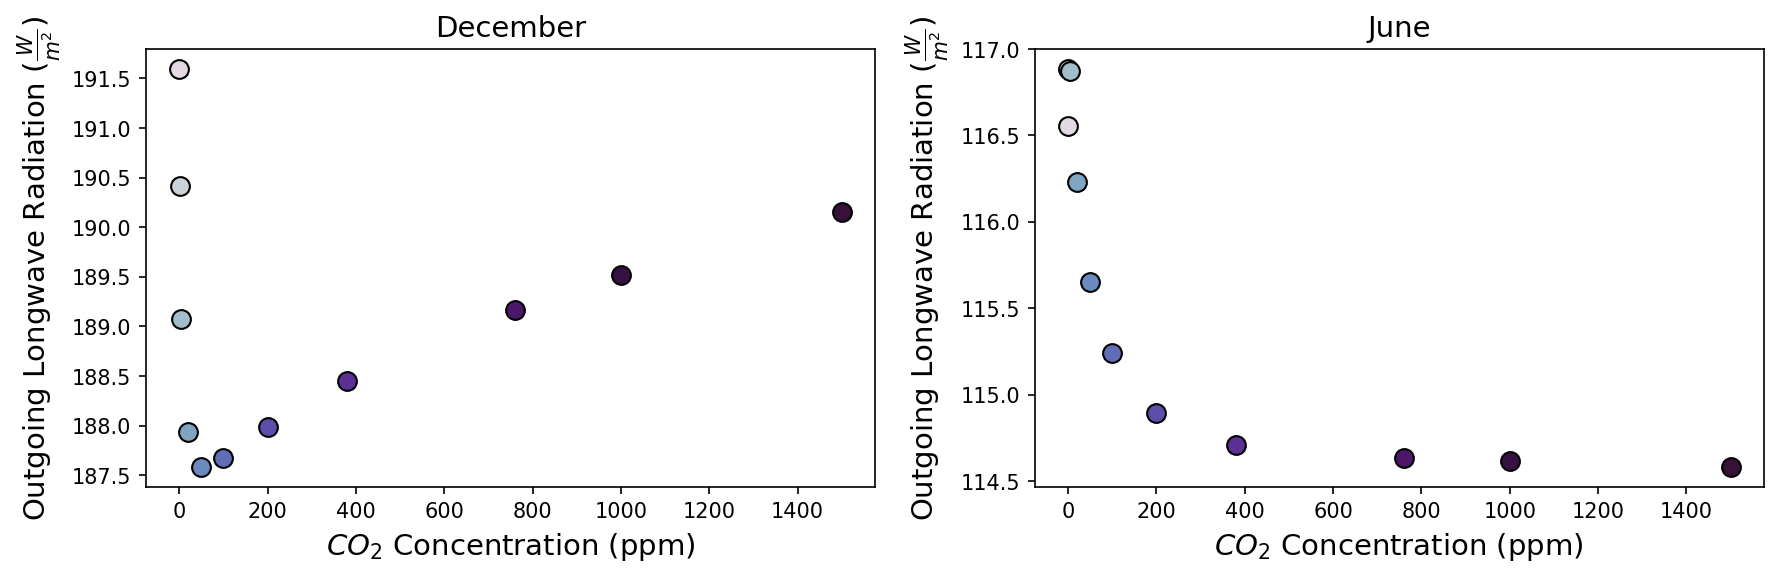
\includegraphics[width=1\textwidth]{figures/OLR_init.png}
\centering
\caption{Initial OLR calculated at our seven different \ce{CO_2} levels in June and December.}
\label{fig:init_OLR}
\end{figure}

This increase in OLR with increasing \ce{CO_2} concentrations leads to increasing TOA radiative loss under higher GHG scenarios during September-April. 

\begin{figure}[htb!]
\noindent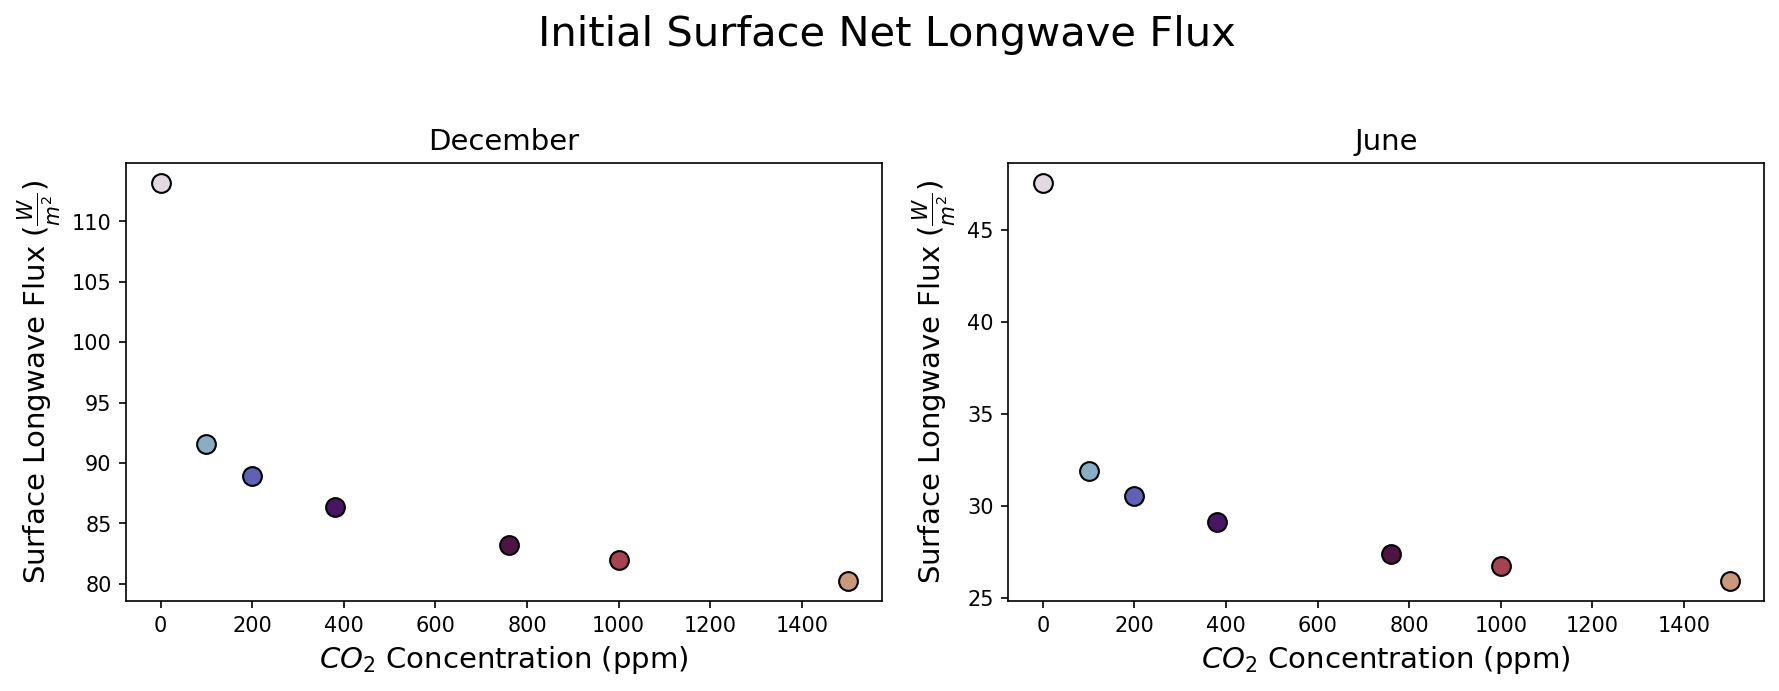
\includegraphics[width=1\textwidth]{figures/sfcLW_init.png}
\centering
\caption{Initial surface net longwave radiation calculated at our seven different \ce{CO_2} levels in June and December.}
\label{fig:init_sfc_LW}
\end{figure}

We find the initial surface net longwave flux decreases with increasing \ce{CO_2} levels across both summer and winter months, as well as the surface net shortwave flux (although it is negligibly small during the winter).  The initial surface upward longwave fluxes are the same across \ce{CO_2} concentrations, as it is calculated by $\sigma*T_s^4$ and the surface temperatures ($T_s$) only vary by month. Thus the surface downward longwave flux is what contributes to the changing net flux, as it increases with a higher optical thickness, and the temperature and level from which it is radiating downwards is closer to the ground at a higher \ce{CO_2} concentration. The surface downward shortwave flux and upward shortwave flux are both impacted by \ce{CO_2} concentration and optical thickness, in which downward flux is increased, and upward flux is decreased, but the overall change is much smaller than longwave. This is because \ce{CO_2} mostly intersects with the longwave infrared (IR) spectra, but has small absorptivity in the shortwave IR range (wavenumbers between 2380-2600 $cm^{-1}$ \citep{mlawer_radiative_1997}. 

Additionally, we calculate the greenhouse effect (GHE) of \ce{CO_2} at our initial timestep \ref{fig:GHE} for each month. We find similar results to that of \citep{schmithusen_how_2015}, in which our February, March and April GHE are negative across all \ce{CO_2} concentrations, and October and September shift from an initial positive GHE to negative as concentrations increase. During both spring and fall months we see the strongest cooling effect of \ce{CO_2}, and overall, the GHE in Antarctica is far smaller than for a standard atmosphere \citep{schmithusen_how_2015}.

\begin{figure}[htb!]
\noindent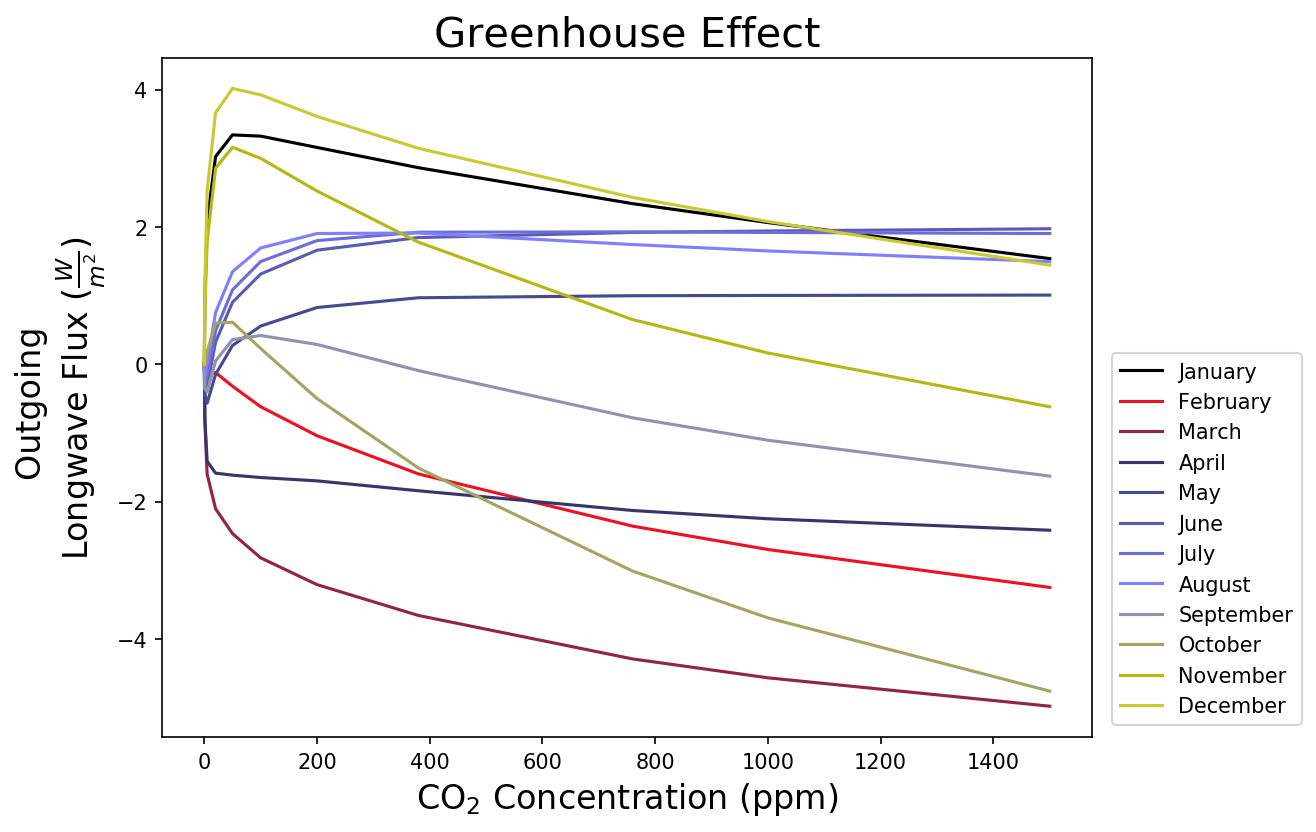
\includegraphics[width=.8\textwidth]{figures/GHE.png}
\centering
\caption{Greenhouse effect of \ce{CO_2} values for each month.}
\label{fig:GHE}
\end{figure}

\subsection{Change over time}
Here we look at the impacts of \ce{CO_2} concentration and season after running the model forward for 3 months, specifically focusing on 380ppm and 760ppm scenarios. 

Surface temperatures increase over time across all months \ref{fig:temp_step} and \ce{CO_2} concentrations. We also find 


\begin{figure}[htb!]
\noindent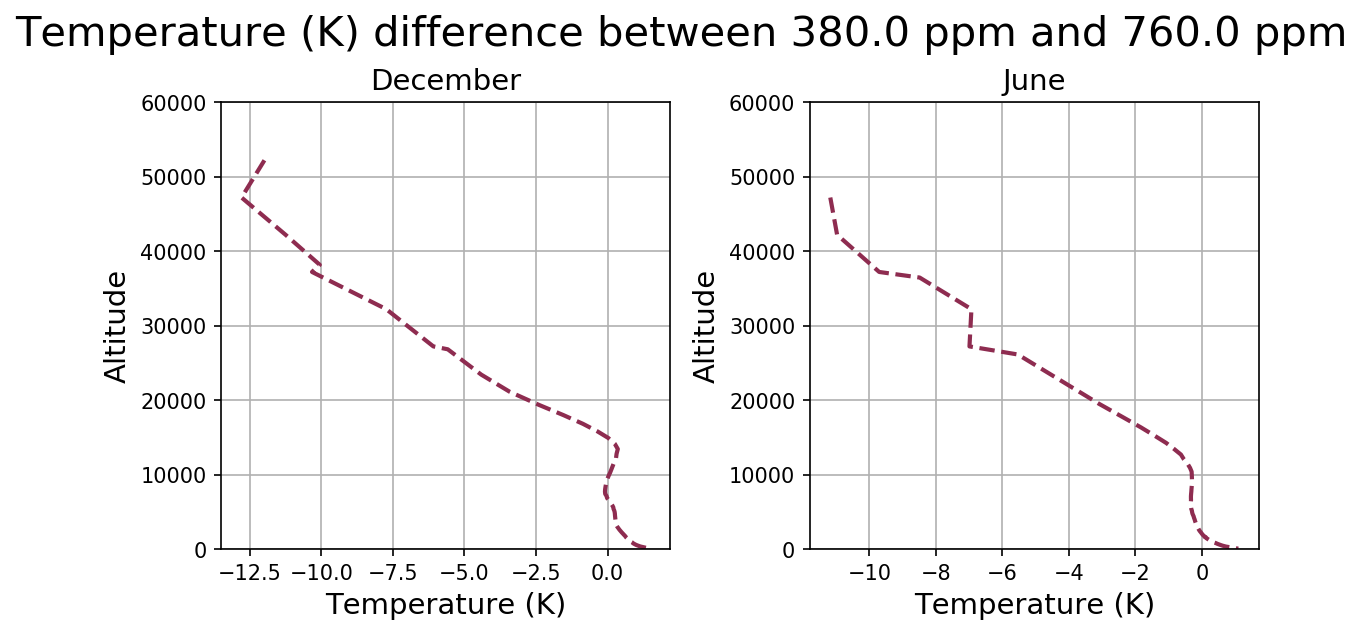
\includegraphics[width=.8\textwidth]{figures/temp_evolution.png}
\centering
\caption{Temperature differences by month and \ce{CO_2} concentration.}
\label{fig:temp_step}
\end{figure}
Our longwave fluxes are also increasing over time, and the resulting heating rates are cooling the atmosphere in both the June and December case, as can be seen in FIGURE****. Shortwave fluxes, on the other hand, are negligibly small in June, but acting to warm the atmosphere in December. The turbulent heating rate cools the lower atmosphere in June and December, aside from the lowest atmospheric level in December, during which it is warming. Lastly, the advection is warming the entire column during June, to counteract the combined cooling of the longwave heating rate and turbulent heating rates. During December, it is more complicated, as the advection cools the lower troposphere to counteract turbulence, and switches between cooling and warming throughout the upper levels of the atmosphere in order to counteract the combined cooling and heating provided by the longwave and shortwave, respectively. This leads to a net heating throughout the atmosphere in all seasons, and thus the warming that we find.

\begin{figure}[htb!]
\noindent
\includegraphics[width=1\textwidth]{figures/ASR_OLR.png}
\centering
\caption{OLR and ASR for 380ppm and 760ppm in December and June over 5 months.}
\label{fig:ASR_OLR}
\end{figure}


Under different \ce{CO_2} concentrations, at our final timestep, we find that the surface temperature warms an additional 1.1\degree of warming during June, and an additional 1.5\degree of warming in December. This supports previous work in the conclusion that the sign of TOA OLR cannot be used to immediately diagnose the surface level temperature response to GHG in the case of the Antarctic. Furthermore, this extends to the atmosphere, as long as we are looking at the combined effects of advection and radiation.

We found, in the initial conditions, that the OLR decreased with \ce{CO_2} during all but the winter months. 

\pagebreak
\bibliographystyle{apalike}
\bibliography{references.bib}

\end{document}

